    
    
    \section{Supplements}
    
    
    % ====================================================================== %
    %                           Stagger/Collocated                           %
    % ====================================================================== %
    \subsection*{Staggered/Collocated}
    \begin{frame}[c,label=Meshes]{Staggered/Collocated}
        \begin{columns}
            \begin{column}[T]{0.4\textwidth}
                Staggered mesh:                
               \begin{center}
                   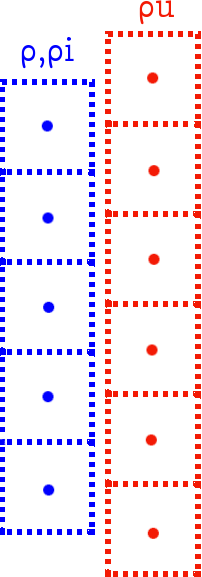
\includegraphics[height=2.2in]{StaggeredMesh}
               \end{center}
            \end{column}
            \hfill
            \begin{column}[T]{0.4\textwidth}
                Collocated mesh:
                \begin{center}
                    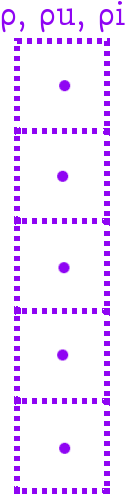
\includegraphics[height=2.2in]{CollocatedMesh}
                \end{center}
            \end{column}
        \end{columns}
    \end{frame}
    
    
    % ====================================================================== %
    %                      Rigorous/Non-rigorous                             %
    % ====================================================================== %
    \subsection*{Rigorous vs. Nonrigorous}
    \begin{frame}[c,label=Nonrigor]{Rigorous vs. Non-Rigorous}\label{Rigorous}
        \begin{columns}
            \begin{column}[T]{0.4\textwidth}
                Rigorous staggered mesh (CFD):                
               \begin{center}
                   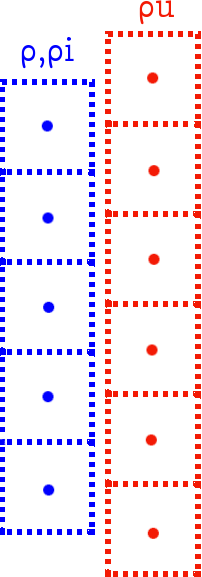
\includegraphics[height=2.2in]{StaggeredMesh}
               \end{center}
            \end{column}
            \hfill
            \begin{column}[T]{0.4\textwidth}
                Non-rigorous staggered mesh (System codes):
                \begin{center}
                    \null\vfill
                    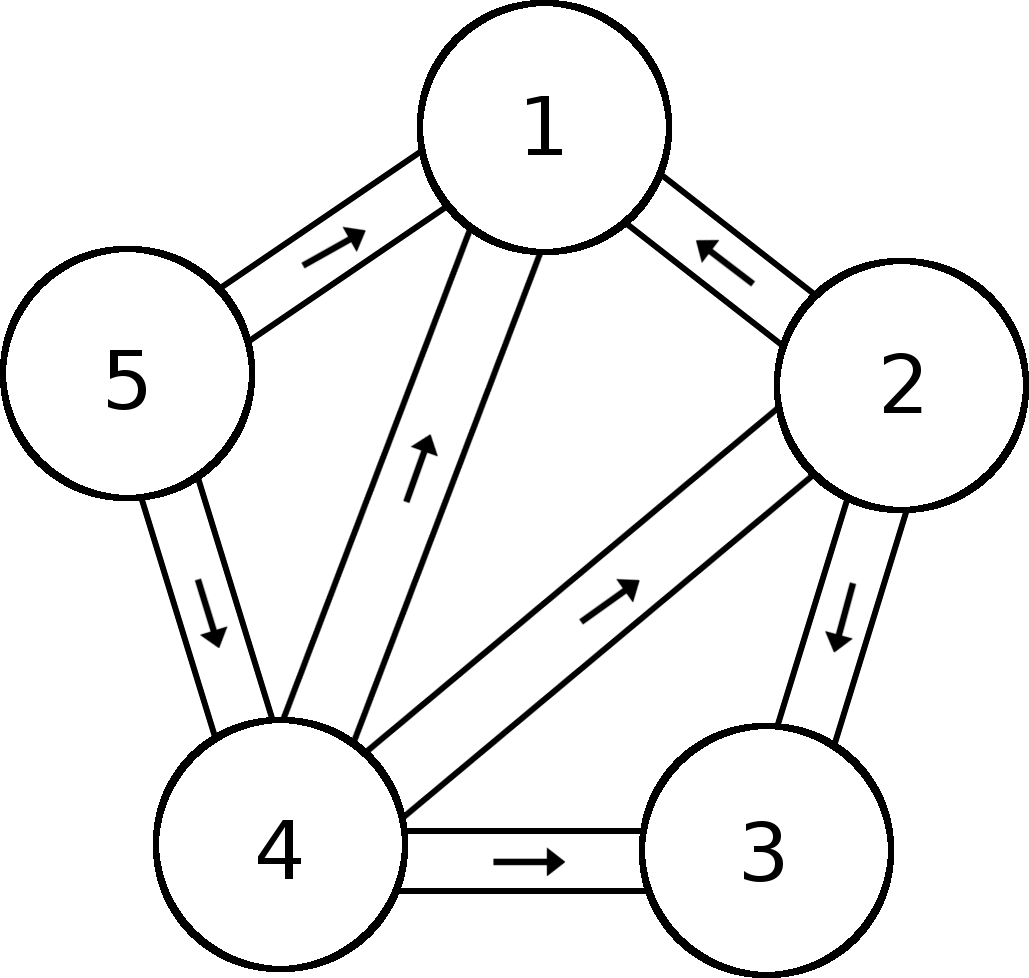
\includegraphics[scale=0.325]{NonrigorousMesh}
                    \null\vfill
                \end{center}
                \hfill\textit{\tiny\hyperlink{NonrigorMain}{return}}
            \end{column}
        \end{columns}
    \end{frame}
    
    
    % ====================================================================== %
    %                          Acoustic Speeds                               %
    % ====================================================================== %
    \subsection*{Acoustic Speeds}
    \begin{frame}[c,label=AcousticSpeeds]{Acoustic Speeds}
       \begin{center}
            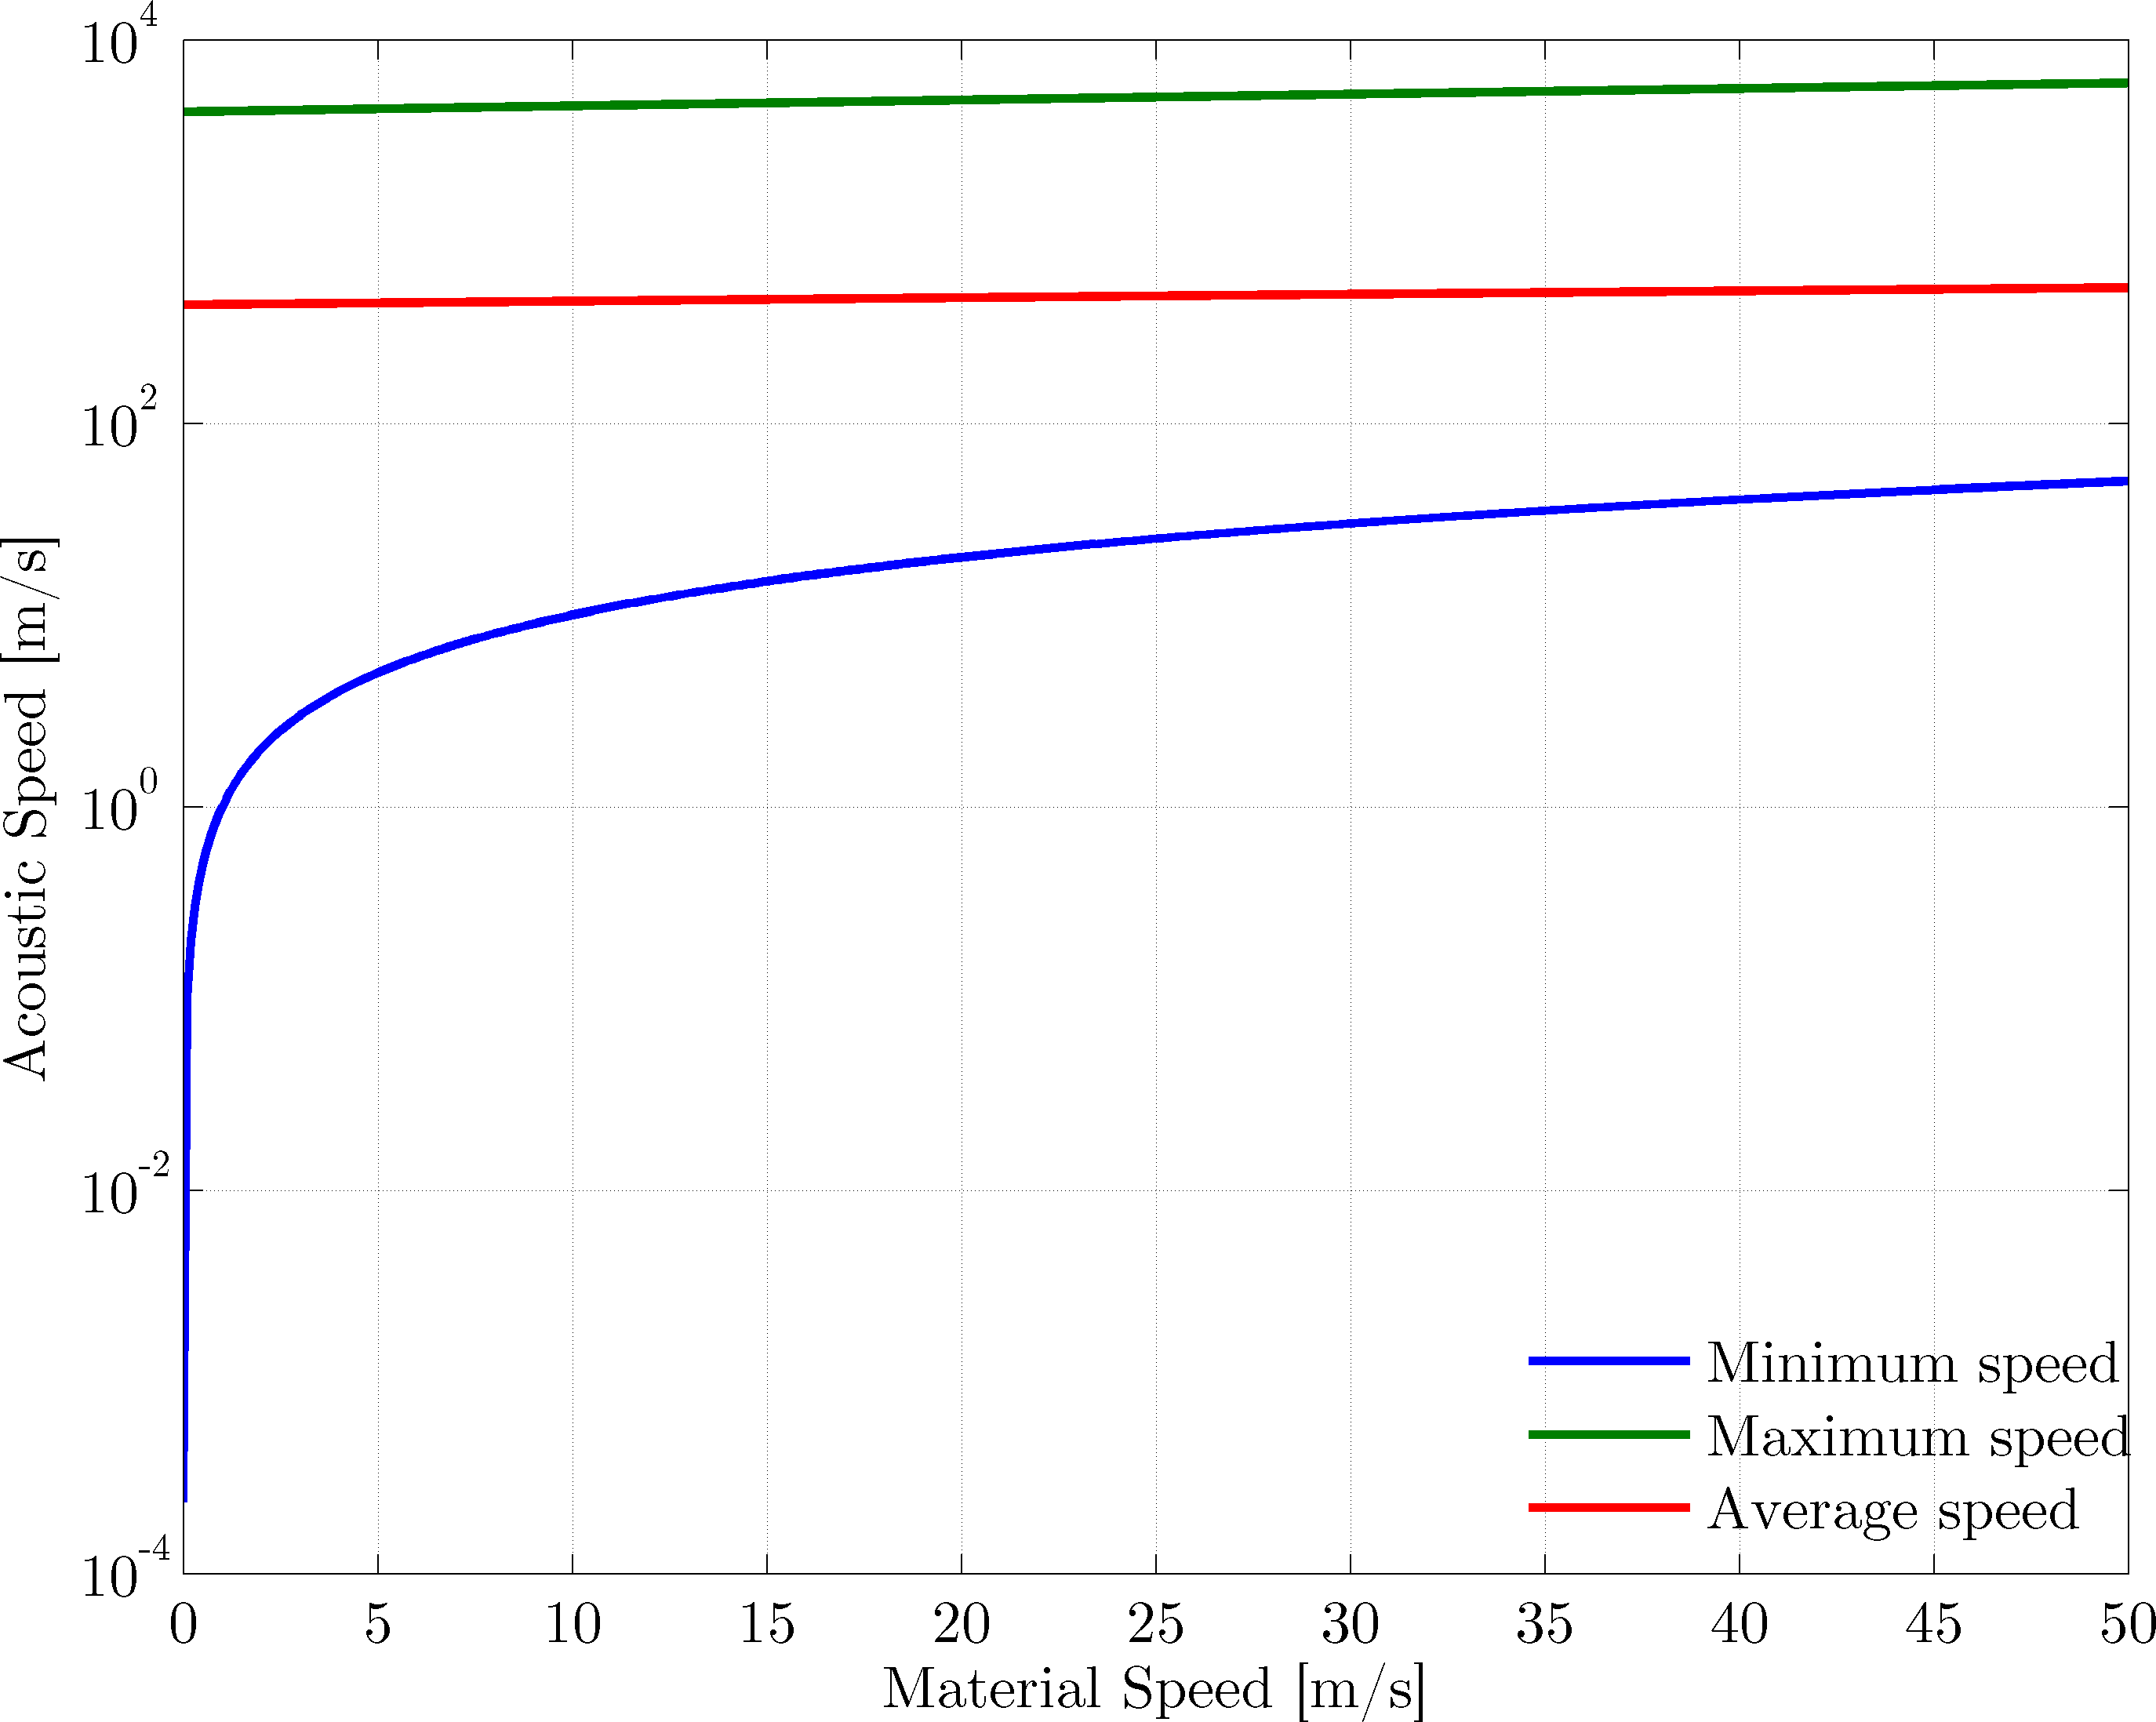
\includegraphics[height=2.2in]{AcousticSpeedVsMaterialSpeed}
       \end{center}
        \hfill\textit{\tiny\hyperlink{AcousticSpeedsMain}{return}}
    \end{frame}



    % ====================================================================== %
    %                          Non-simple, closed loop                       %
    % ====================================================================== %
    \subsection*{Non-simple, closed loop}
    \begin{frame}[c,label=NonsimpleClosedLoop]{Non-simple, closed loop}
        \begin{center}
            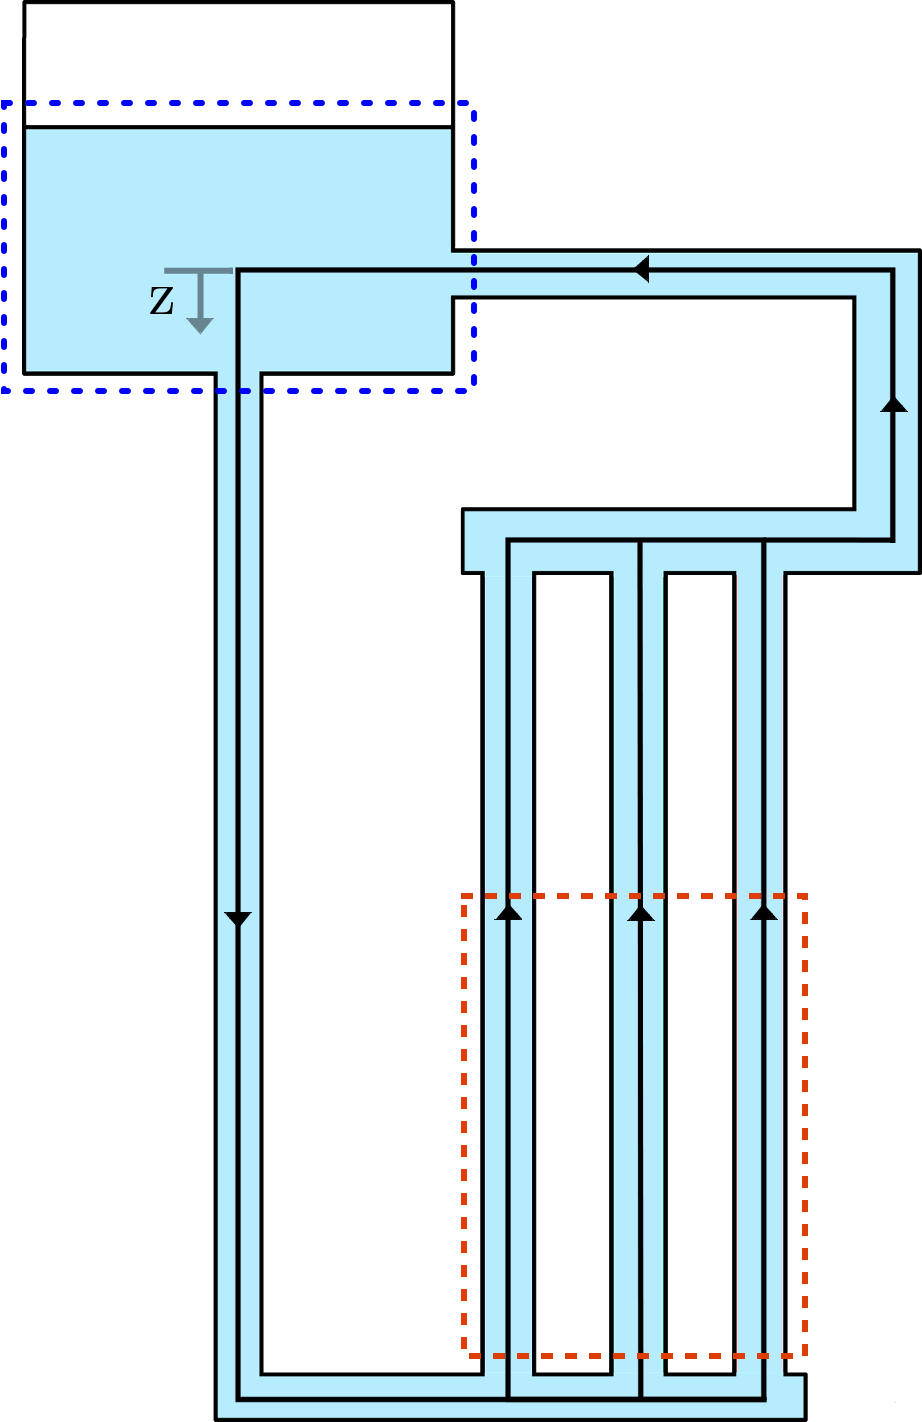
\includegraphics[height=2.2in]{ComputationalGeometry}
        \end{center}
    \end{frame}
    
    
    % ====================================================================== %
    %                          Non-simple, closed loop                       %
    % ====================================================================== %
    \subsection*{i-rho Space}
    \begin{frame}[c,label=irhoSpace]{$i$-\rho Diagram}
        \begin{center}
            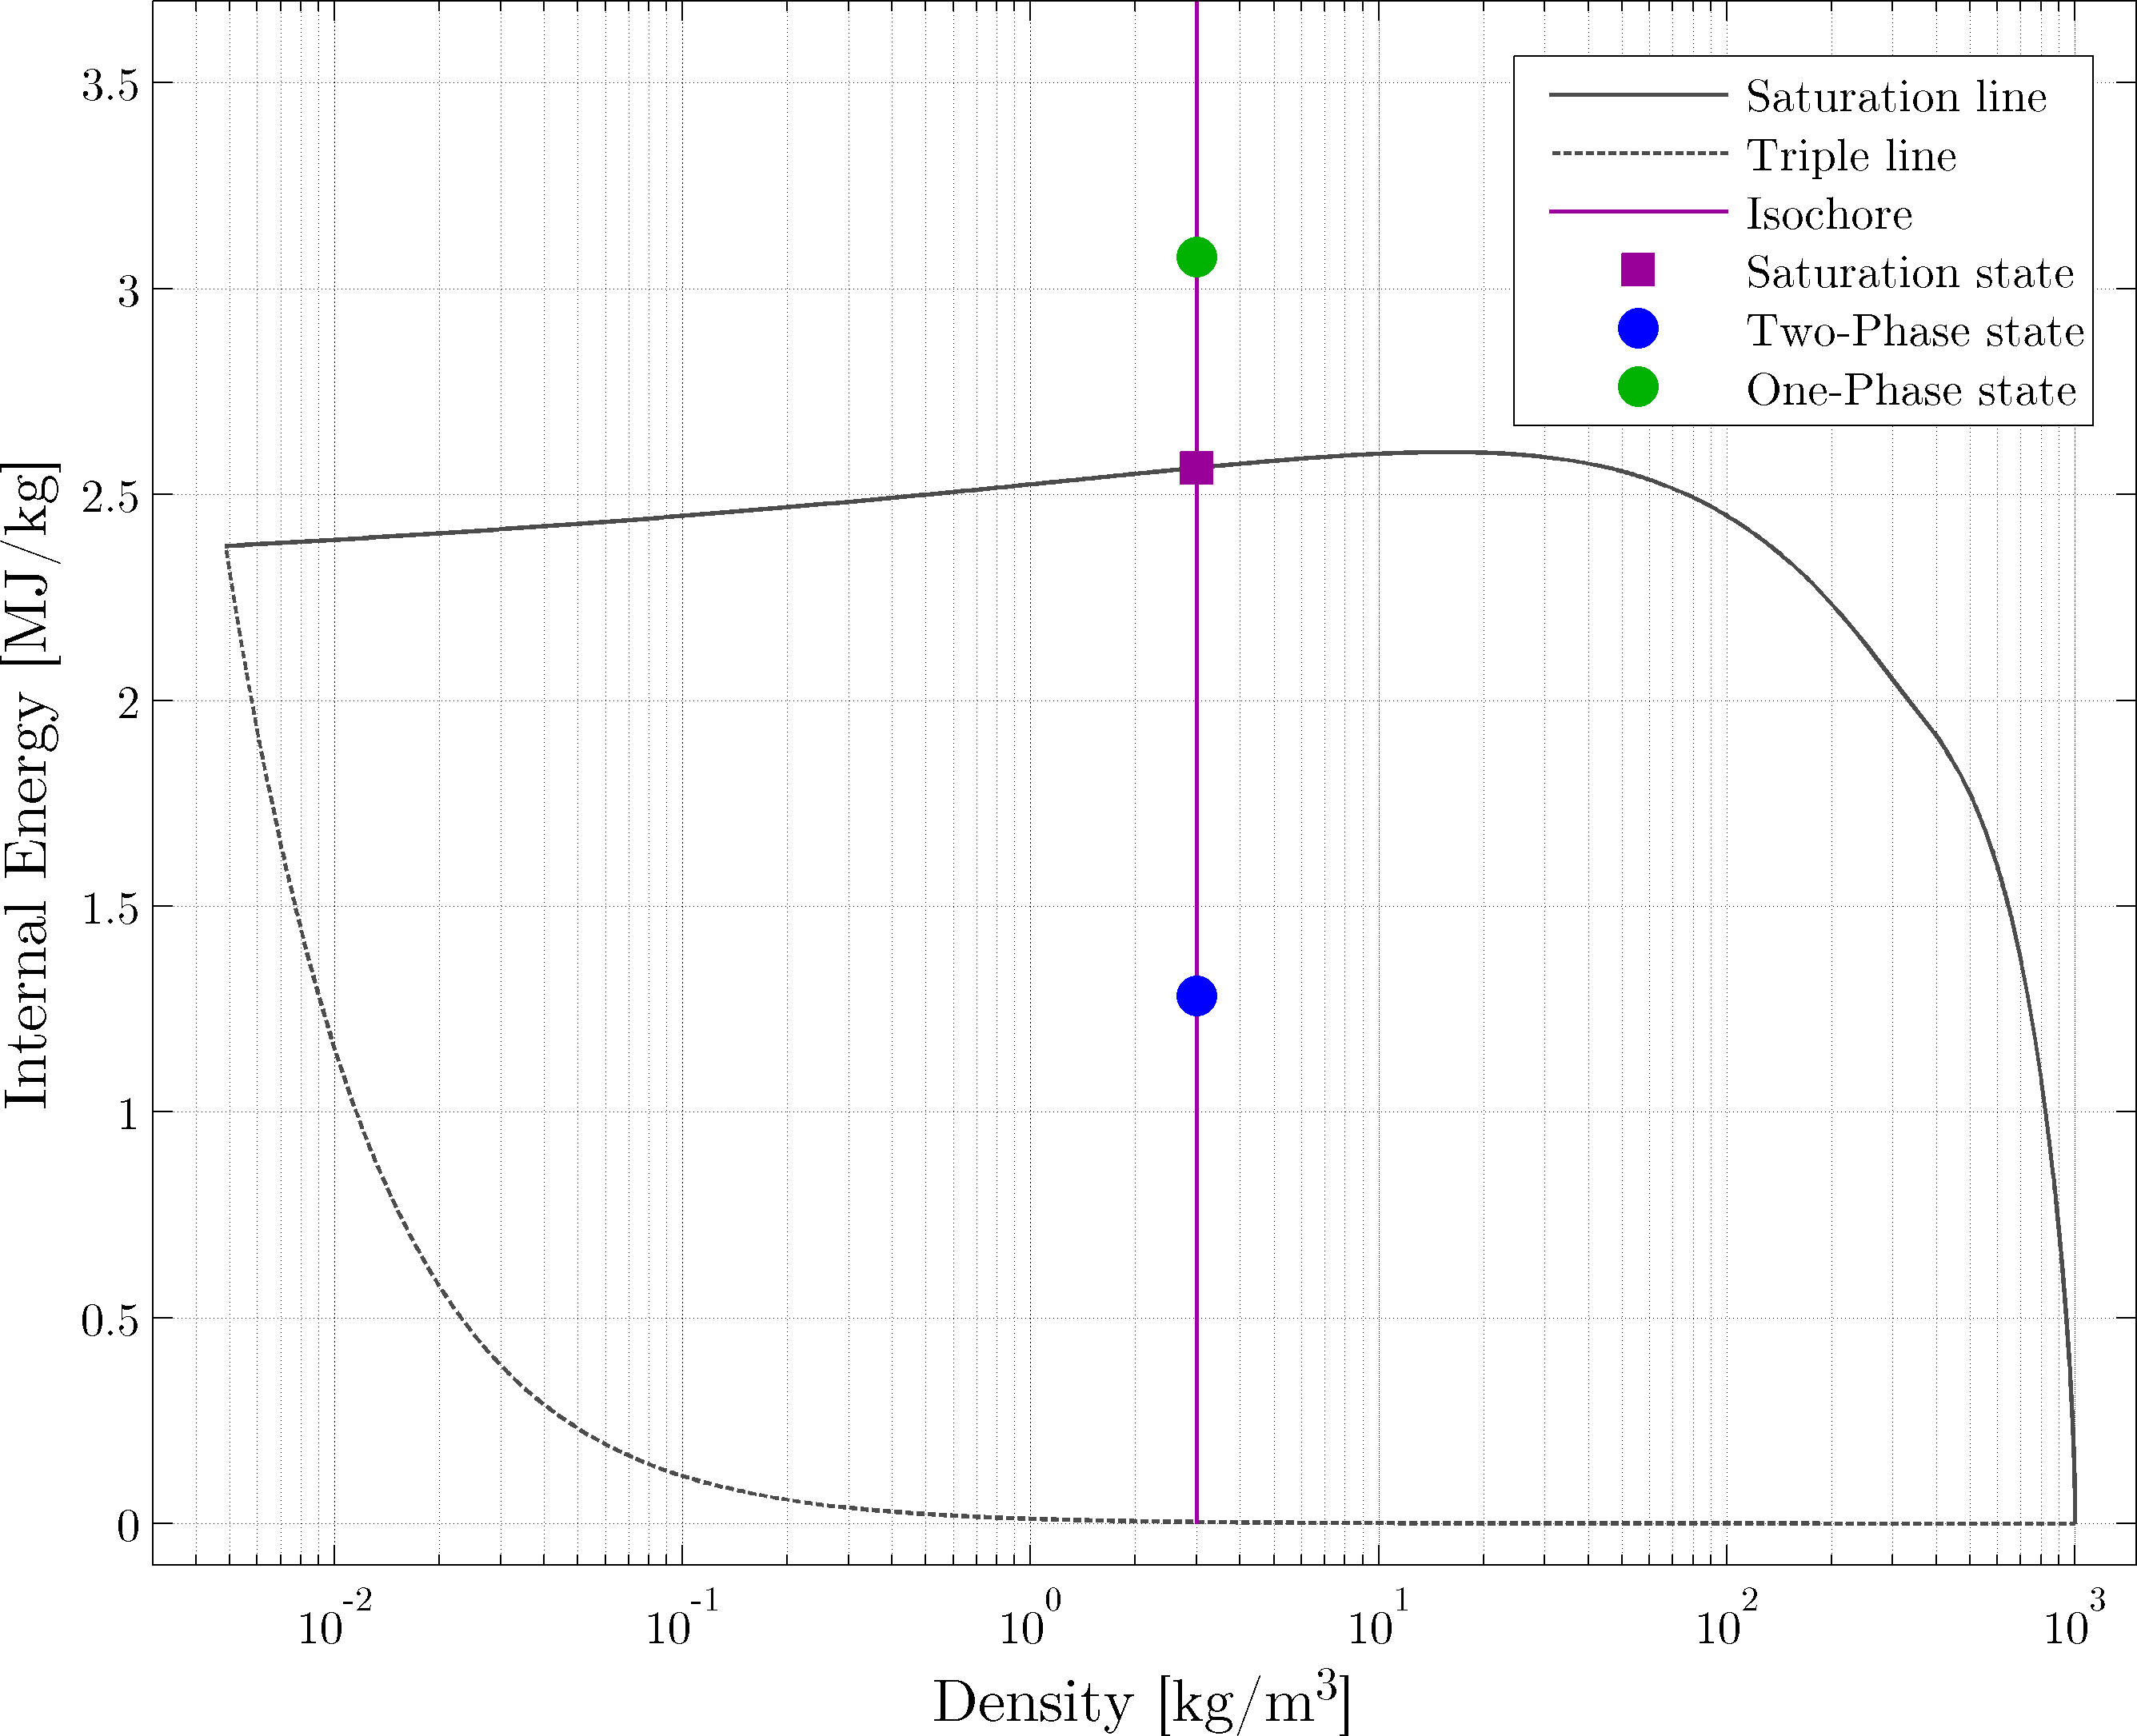
\includegraphics[height=2.2in]{InteEnergyVsDensity}
        \end{center}
        \hfill\textit{\tiny\hyperlink{EOS}{return}}
    \end{frame}
    
    
    
    % ====================================================================== %
    %                            Stability Diagrams                          %
    % ====================================================================== %
    \subsection*{Stability Diagrams}
    \begin{frame}[c,label=StabilityDiagrams]{Stability Diagrams}
        \begin{columns}
            \begin{column}[T]{0.4\textwidth}
                Linearly stable, nonlinearly unstable:
                \begin{center}
                    \vspace{0.09in}
                    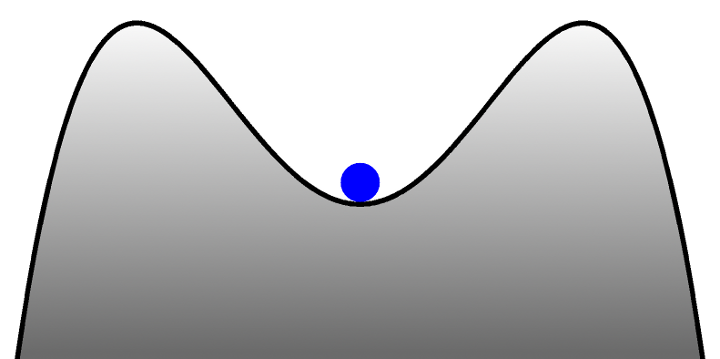
\includegraphics[height=0.91in]{LinearlyStableNonlinearlyUnstable}
                \end{center}
            \end{column}
            \hfill
            \begin{column}[T]{0.4\textwidth}
                Linearly unstable, nonlinearly stable:
                \begin{center}
                    \null\vfill
                    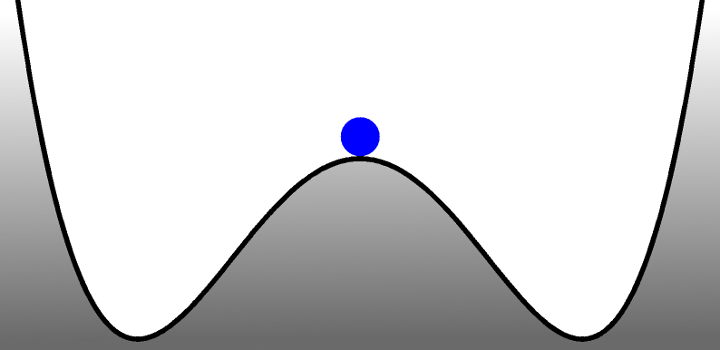
\includegraphics[height=0.83in]{LinearlyUnstableNonlinearlyStable}
                    \null\vfill
                \end{center}
                \hfill\textit{\tiny\hyperlink{Perturbation}{return}}
            \end{column}
        \end{columns}
    \end{frame} 
    
    
    
    % ====================================================================== %
    %                            Stability Diagrams                          %
    % ====================================================================== %
    \subsection*{System Mass flow: 4 days}
    \begin{frame}[c,label=MassFlow4Days]{System Mass flow: 4 days}
        \begin{center}
            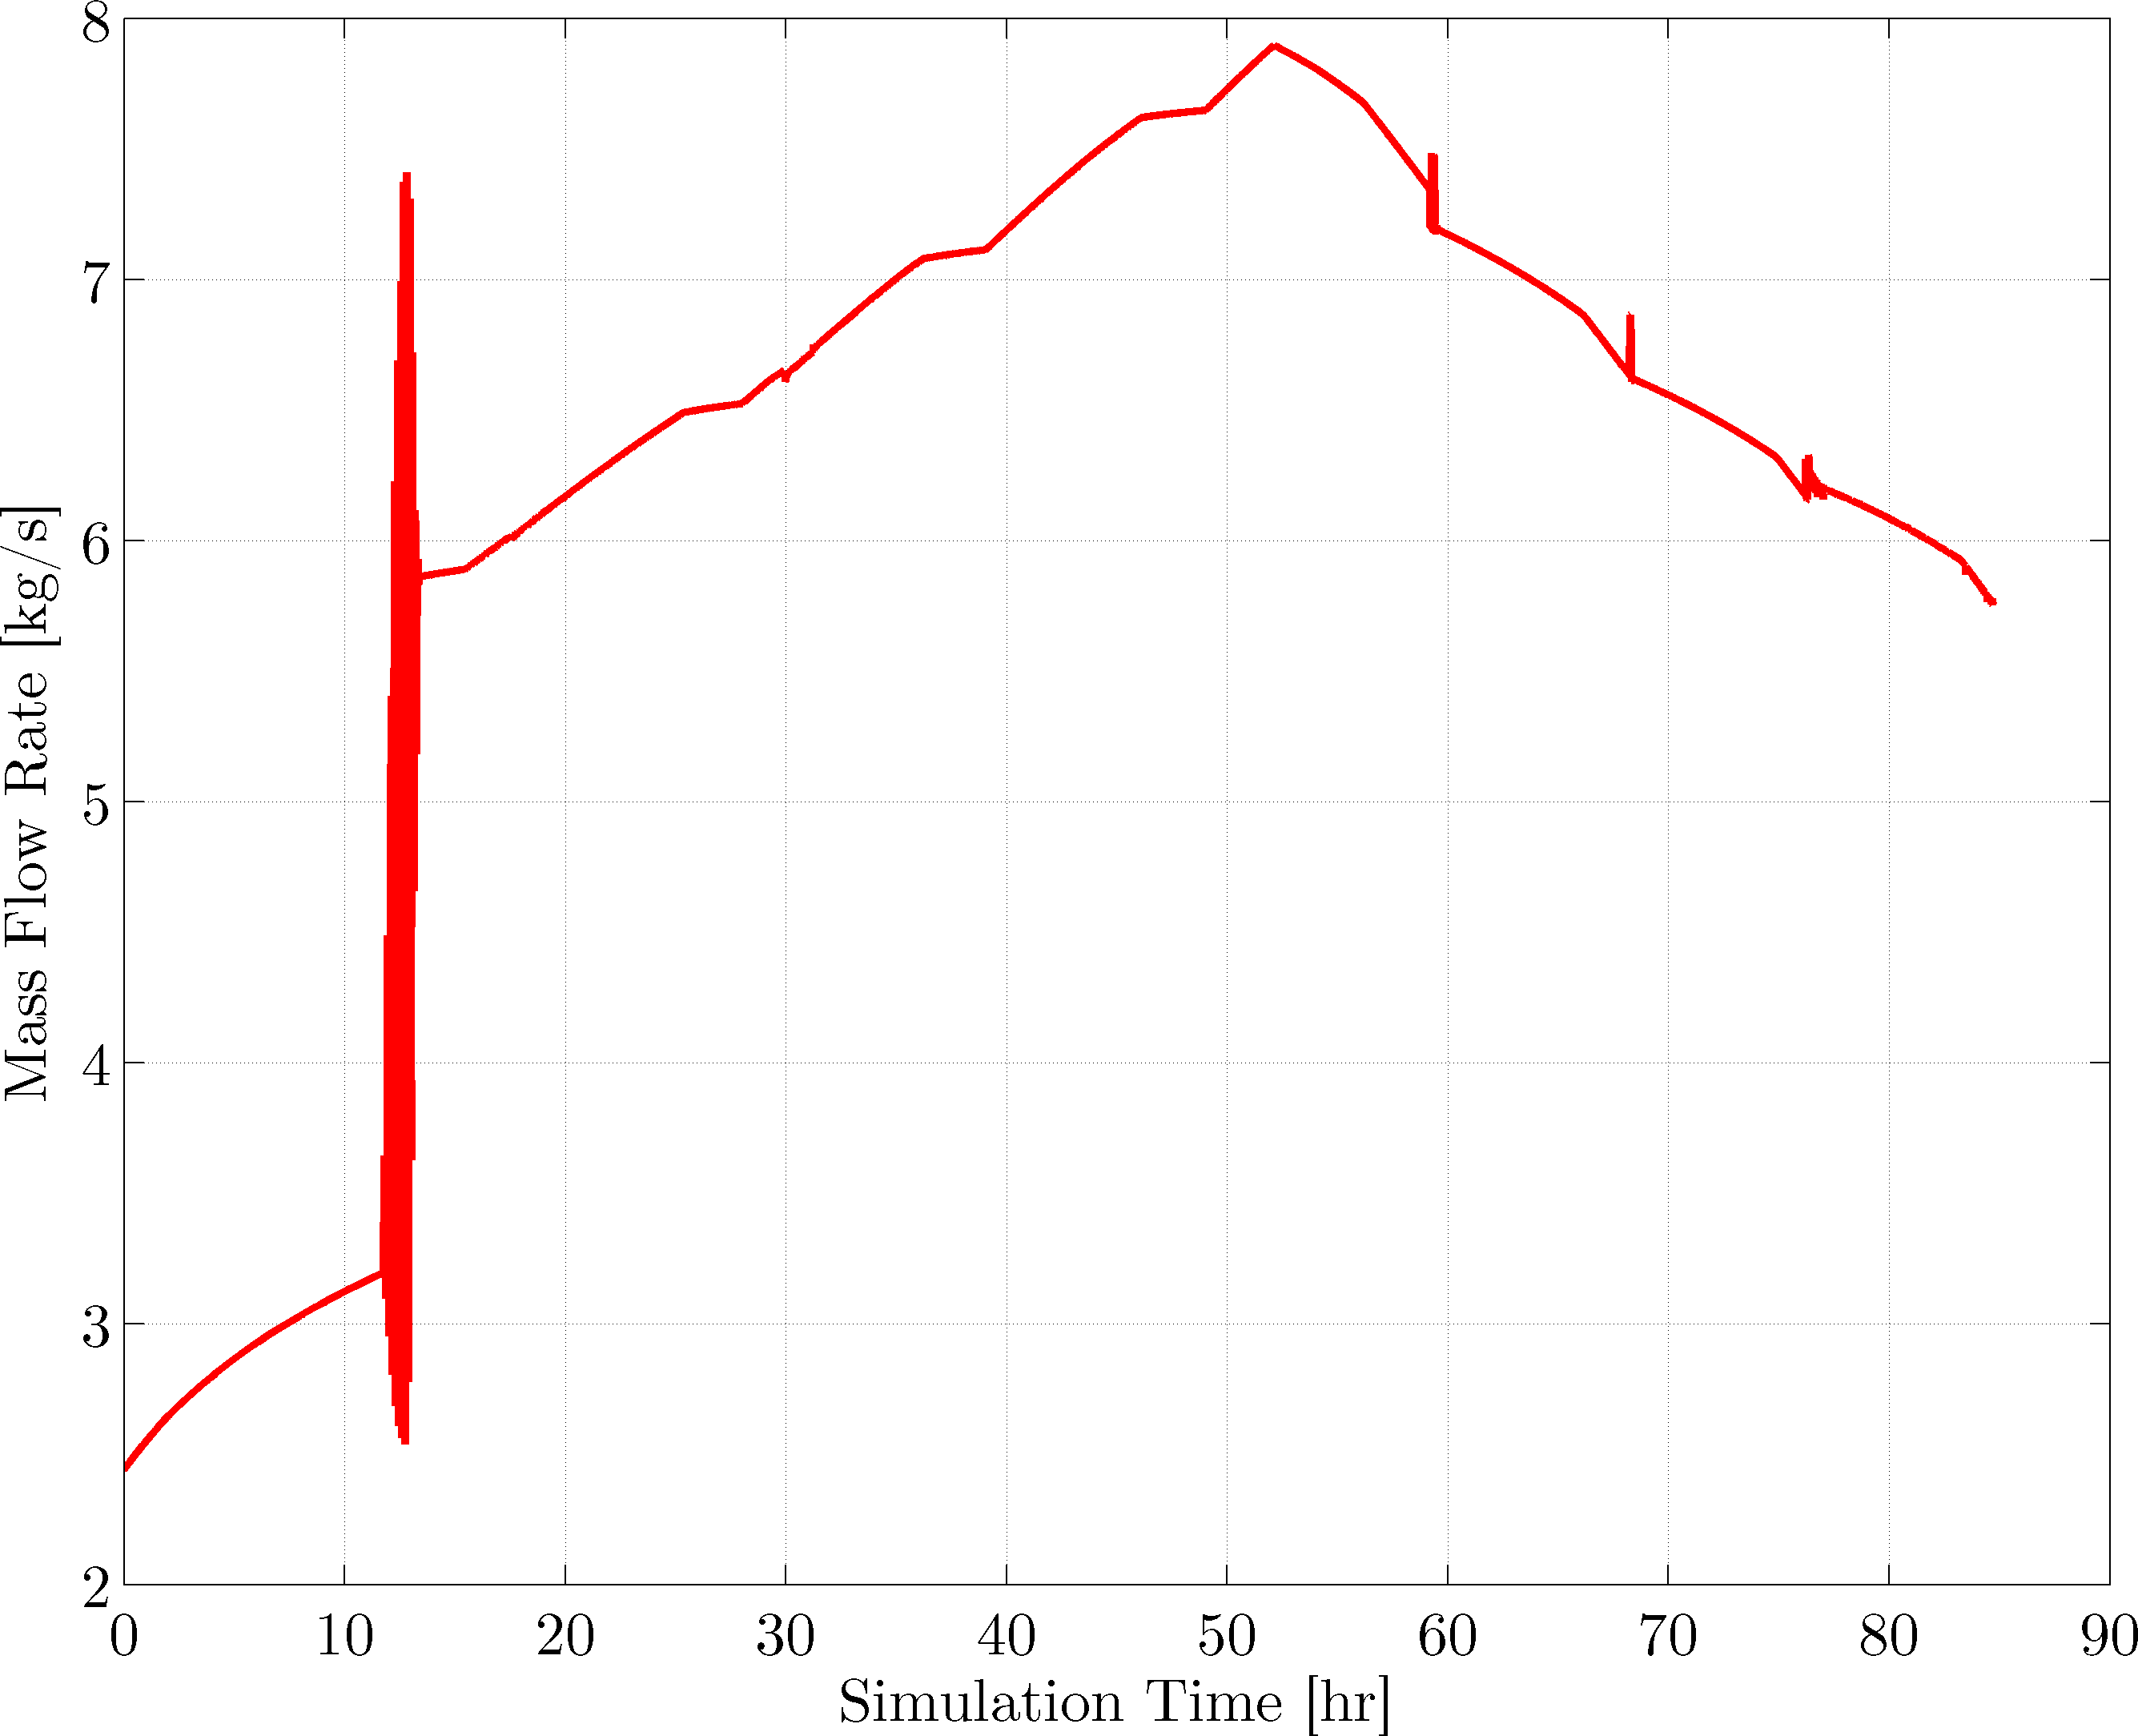
\includegraphics[height=2.4in]{MassRateFor4days}
        \end{center}
        \hfill\textit{\tiny\hyperlink{MassFlowAnnotate}{return}}
    \end{frame}
    
    
    
    % ====================================================================== %
    %                             Multiphase Model                           %
    % ====================================================================== %
    \subsection*{Multiphase Model}
    \begin{frame}[label=Multiphase]{Multiphase Model}
         \begin{equation}
            \renewcommand{\arraystretch}{2.2}
            \pderiv{}{t}\begin{bmatrix}
                           \rhok \\
                           \rhouk \\
                           \rhoik 
                        \end{bmatrix}
            + 
            \pderiv{}{z}\begin{bmatrix}
                            \rhouk                 \\
                            \uk\,    \rhouk  + P(\rho\subs{\phi},\ik)   \\
                            \uk\left[\rhoik  + P(\rho\subs{\phi},\ik)\right]
                        \end{bmatrix}
                     = 
        \end{equation}
        \begin{equation}\renewcommand{\arraystretch}{2.2}
            \begin{bmatrix}
                \mathbb{M}\subs{\phi} \\
                \rhok{g(z)} - \frac{K_{\text{eff,$\phi$}}(\qCon)}{2} \uk\,|\rhouk| + \mathbb{P}\subs{\phi}  \\
                \dot{Q}\subs{add,\phi}(\qCon,z,t) + \mathbb{E}\subs{\phi}
            \end{bmatrix}
            \notag
        \end{equation}
    \end{frame}
